% ==============================================================================
% Modelo de Trabalho de Conclusão de Curso (TC) - Ciência da Computação (CIC)
% Instituto de Informática - Universidade Federal do Rio Grande do Sul (UFRGS)
% Padrão: iiufrgs.cls / ABNT (NBR 14724, NBR 6023, NBR 10520, NBR 6027)
% Compatível com Overleaf e TeX Live moderno (biblatex + biber)
% ==============================================================================
\documentclass[cic,tc,biblatex]{iiufrgs}

% Opções comuns da classe iiufrgs:
%   * cic       -- Curso de Ciência da Computação
%   * ecp       -- Curso de Engenharia de Computação
%   * ppgc      -- Pós-Graduação em Computação
%   * pgmicro   -- Pós-Graduação em Microeletrônica
%   * tc / dipl -- Trabalho de Conclusão de Curso (graduação)
%   * diss / mestrado -- Dissertação de Mestrado
%   * tese / doutorado -- Tese de Doutorado
%   * biblatex  -- Utiliza biblatex + biber + estilo ABNT (recomendado)
%   * abntex2cite -- Utiliza bibtex legado com abntex2-alf.bst
%   * english   -- Redige o documento em inglês (inverte ordem dos resumos)
%   * openright -- Força que todo capítulo inicie em página ímpar (padrão de livros)
%   * oneside   -- Configuração somente frente (omite formatação frente-e-verso)

% Arquivo contendo as referências bibliográficas
\addbibresource{biblio.bib}

% Pacotes recomendados para recursos adicionais
\usepackage{booktabs}       % Tabelas com acabamento profissional (\toprule, \midrule, \bottomrule)
\usepackage{amsmath,amssymb} % Fórmulas e símbolos matemáticos avançados
\usepackage{listings}       % Listagens de código-fonte
\usepackage{microtype}      % Ajuste tipográfico fino de espaçamento

% Configuração de formatação para trechos de código (listings)
\lstset{
    basicstyle=\ttfamily\small,
    keywordstyle=\bfseries,
    numbers=none,
    frame=single,
    breaklines=true,
    captionpos=t,
    tabsize=2,
    showstringspaces=false
}

% ------------------------------------------------------------------------------
% Informações Gerais do Trabalho (Metadados da Capa e Folha de Rosto)
% ------------------------------------------------------------------------------
\title{Guia e Modelo de Trabalho de Conclusão em Ciência da Computação}
\translatedtitle{Guide and Template for Graduation Projects in Computer Science}

% Autor: {Sobrenome}{Nome(s)}
\author{da Silva}{João}
% Em trabalhos com múltiplos autores, repita o comando:
%\author{Sobrenome}{Nome}

% Dica: dúvidas sobre acentuação e partículas em nomes de autores (ex: von, de, da)?
% Consulte: https://www.ime.usp.br/~tassio/TMP/latex-mooc/material/partes-dos-nomes.pdf

% Orientador(a): [Titulação]{Sobrenome}{Nome(s)}
\advisor[Prof.~Dr.]{Sobrenome}{Nome}
% Coorientador(a) (opcional):
%\coadvisor[Prof\textsuperscript{a}.~Dra.]{Sobrenome}{Nome}

% Palavras-chave na língua do documento (até 10, com primeira letra maiúscula)
\keyword{Trabalho de conclusão de curso}
\keyword{Metodologia científica}
\keyword{Formatação de documentos}
\keyword{\LaTeX}
\keyword{UFRGS}

% Palavras-chave na língua estrangeira
\translatedkeyword{Graduation project}
\translatedkeyword{Scientific methodology}
\translatedkeyword{Document preparation}
\translatedkeyword{\LaTeX}
\translatedkeyword{UFRGS}

% Local e data (mês/ano correntes por padrão, ou force com \date{mês}{ano})
%\location{Porto Alegre}{RS}
%\date{novembro}{2026}

% ------------------------------------------------------------------------------
% Nominata Institucional (Personalização Dinâmica de Gestão)
% ------------------------------------------------------------------------------
% Os cargos da administração (Reitora, Pró-Reitor, Diretor do II, Coordenador etc.)
% são definidos centralizadamente em `nominata.def` e associados dinamicamente ao curso
% escolhido (`cic.def`, `ecp.def`, etc.).
% Caso ocorram alterações em cargos de gestão, você pode:
%   a) Atualizar diretamente o arquivo `nominata.def`;
%   b) Ou redefinir comandos específicos aqui no preâmbulo com \renewcommand:
%      \renewcommand{\nominataCoord}{Prof.~Nome Sobrenome}
%      \renewcommand{\nominataCoordname}{Coordenador do Curso de Ciência de Computação}
%      \renewcommand{\nominataDir}{Prof.~Nome Sobrenome}
%      \renewcommand{\nominataReit}{Prof\textsuperscript{a}.~Nome Sobrenome}
%   c) Ou criar um arquivo `nominatalocal.def` e passar a opção [nominatalocal] na classe.
% ------------------------------------------------------------------------------

\begin{document}

% ==============================================================================
% 1. ELEMENTOS PRÉ-TEXTUAIS
% ==============================================================================
% A norma ABNT NBR 14724 divide o trabalho em:
%   - Pré-textuais: folha de rosto, dedicatória, agradecimentos, resumos, listas e sumário
%   - Textuais: introdução, desenvolvimento (trabalhos relacionados, fundamentação,
%     proposta, metodologia, avaliação/experimentos) e conclusão
%   - Pós-textuais: referências, apêndices e anexos
% ==============================================================================

% Produz a folha de rosto e a folha de nominata/aprovação
\maketitle

% Dedicatória (opcional): elemento não titulado, alinhado à direita na base da página
\begin{dedicatoria}
\textit{Dedico este trabalho a ...\\}
\end{dedicatoria}

% Agradecimentos (opcional): elemento com título centralizado não numerado
\begin{agradecimentos}
Agradeço à Universidade Federal do Rio Grande do Sul e ao Instituto de Informática por proporcionarem um ambiente de excelência acadêmica.

Ao meu orientador/a pela ...

Aos colegas de curso e amigos pelo ...
\end{agradecimentos}

% Resumo na língua vernácula (obrigatório):
% Deve ser composto por parágrafo único (de 150 a 500 palavras), redigido em voz ativa
% e terceira pessoa. Deve ressaltar sucintamente o objetivo, o método, os resultados
% e as conclusões do documento. As palavras-chave são inseridas automaticamente ao final.
\begin{abstract}
Este modelo tem o objetivo de orientar alunos do Curso de Ciência da Computação (CIC) do Instituto de Informática da UFRGS na estruturação de seus Trabalhos de Conclusão (TC), apresentando tanto as diretrizes metodológicas de organização de conteúdo quanto o uso prático dos recursos tipográficos em \LaTeX. São descritas as funções dos elementos pré-textuais, textuais e pós-textuais de acordo com as normas da Associação Brasileira de Normas Técnicas (ABNT) e as diretrizes do II/UFRGS. Adicionalmente, exemplifica-se a elaboração de cada capítulo do trabalho acadêmico (introdução, trabalhos relacionados, fundamentação teórica, desenvolvimento metodológico, experimentação/avaliação e conclusões), bem como a correta inserção de figuras, tabelas, equações, códigos-fonte e referências bibliográficas utilizando o moderno sistema \textsf{biblatex} com motor \textsf{biber}. Com este guia, espera-se agilizar a redação do trabalho acadêmico, assegurar a consistência visual e elevar o rigor formal do texto científico.
\end{abstract}

% Resumo em língua estrangeira (obrigatório):
% Tradução fidedigna do resumo para o inglês (ou língua estrangeira correspondente).
\begin{translatedabstract}
This template aims to guide undergraduate Computer Science students at the Institute of Informatics (UFRGS) in structuring their Graduation Projects (TC), presenting methodological content organization guidelines and practical typesetting examples in \LaTeX. It describes the role of pre-textual, textual, and post-textual elements according to the Brazilian National Standards Organization (ABNT) and institutional regulations. Furthermore, it exemplifies how to write each core chapter of an academic monograph (introduction, related work, background, development, experimental evaluation, and conclusions), alongside best practices for including figures, tables, equations, source code snippets, and bibliographic citations with modern \textsf{biblatex} and \textsf{biber}. By using this guide, students can streamline thesis preparation while ensuring high typographic consistency and scientific rigor.
\end{translatedabstract}

% Lista de Figuras (opcional, recomendada quando houver ilustrações)
\listoffigures

% Lista de Tabelas (opcional, recomendada quando houver tabelas)
\listoftables

% Lista de Abreviaturas e Siglas (opcional):
% O parâmetro inicial deve ser a sigla mais longa para calcular o recuo horizontal.
% Conforme a NBR 14724, as siglas devem ser apresentadas em ordem alfabética.
\begin{listofabbrv}{SGBD}
    \item[ABNT] Associação Brasileira de Normas Técnicas
    \item[API]  \emph{Application Programming Interface}
    \item[CIC]  Curso de Ciência da Computação
    \item[IA]   Inteligência Artificial
    \item[II]   Instituto de Informática
    \item[PLN]  Processamento de Linguagem Natural
    \item[SGBD] Sistema de Gerenciamento de Banco de Dados
    \item[TC]   Trabalho de Conclusão
    \item[UFRGS] Universidade Federal do Rio Grande do Sul
\end{listofabbrv}

% Sumário (obrigatório):
% Conforme a ABNT NBR 6027, deve ser o último elemento pré-textual.
\tableofcontents

% ==============================================================================
% 2. ELEMENTOS TEXTUAIS
% ==============================================================================

\chapter{Introdução}
\label{cap:introducao}

A introdução é a porta de entrada do trabalho científico. Sua função principal é contextualizar o tema, definir com clareza o problema investigado e delimitar o escopo da pesquisa para o leitor.

\section{Contextualização e Motivação}
\label{sec:contexto}

Nesta seção inicial, o autor deve apresentar o panorama no qual o trabalho se insere, destacando sua relevância científica, tecnológica ou social. Deve-se responder à pergunta: \emph{``Por que esse tema é importante e merece atenção?''}.

Por exemplo, no campo de Ciência da Computação, pode-se contextualizar o crescimento do volume de dados em redes sociais, a necessidade de processamento em tempo real de grafos de conhecimento~\cite{kg_neo4j} ou os avanços em modelos de linguagem para responder perguntas~\cite{Su2019, wei2022chain}.

\section{Definição do Problema}
\label{sec:problema}

Após contextualizar a área, deve-se afunilar o texto para o \textbf{problema específico} que o trabalho busca responder ou contornar. Seja preciso:
\begin{itemize}
    \item Qual é a lacuna, gargalo, limitação teórica ou deficiência prática encontrada nas soluções atuais?
    \item Quais são os desafios computacionais associados (por exemplo, complexidade de tempo, consumo de memória, interpretabilidade ou alucinações em modelos generativos~\cite{xu2024hallucination})?
\end{itemize}

\section{Objetivos}
\label{sec:objetivos}

Os objetivos definem o compromisso formal do estudante com o leitor e com a banca examinadora.

\subsection{Objetivo Geral}
O objetivo geral resume, em um único parágrafo conciso iniciado por verbo no infinitivo (ex.: \emph{projetar}, \emph{desenvolver}, \emph{avaliar}, \emph{investigar}), a contribuição central do trabalho.

\subsection{Objetivos Específicos}
Os objetivos específicos detalham as metas intermediárias necessárias para atingir o objetivo geral. Recomenda-se apresentá-los em itens:
\begin{enumerate}
    \item Mapear e comparar sistematicamente os trabalhos correlatos existentes na literatura;
    \item Formular a modelagem do sistema ou arcabouço conceitual proposto;
    \item Implementar um protótipo funcional em linguagem adequada;
    \item Conduzir experimentos empíricos com bases de dados de referência para mensurar o desempenho da solução frente a abordagens clássicas.
\end{enumerate}

\section{Estrutura da Monografia}
\label{sec:estrutura_mono}

Ao final da introdução, é boa prática descrever sucintamente o roteiro de leitura dos capítulos subsequentes:
\begin{itemize}
    \item O Capítulo~\ref{cap:relacionados} discute os trabalhos relacionados e o estado da arte;
    \item O Capítulo~\ref{cap:fundamentacao} estabelece a fundamentação teórica indispensável;
    \item O Capítulo~\ref{cap:metodologia} detalha o desenvolvimento e a arquitetura proposta;
    \item O Capítulo~\ref{cap:experimentos} expõe o ambiente experimental, métricas e análise dos resultados;
    \item O Capítulo~\ref{cap:conclusao} conclui o documento com considerações finais e trabalhos futuros.
\end{itemize}

% ------------------------------------------------------------------------------
\chapter{Trabalhos Relacionados}
\label{cap:relacionados}

O capítulo de trabalhos relacionados (ou estado da arte) comprova a maturidade bibliográfica do aluno e contextualiza como a solução proposta se posiciona perante a literatura especializada.

\section{Critérios de Comparação}
Não limite este capítulo a um mero resumo empilhado de resumos de artigos. É essencial adotar uma postura crítica:
\begin{enumerate}
    \item Identificar as premissas, forças e fragilidades de cada abordagem existente;
    \item Sintetizar as semelhanças e contrastes em relação ao seu próprio trabalho;
    \item Resumir a comparação através de uma tabela sintética no final do capítulo.
\end{enumerate}

\section{Exemplo de Citações segundo a ABNT}
\label{sec:citacoes_abnt}

A classe \texttt{iiufrgs} integra-se nativamente ao \textsf{biblatex} com o estilo \textsf{abnt}. A norma NBR~10520 da ABNT estabelece diretrizes rigorosas para a apresentação de citações em documentos acadêmicos. É fundamental distinguir as diferentes modalidades de citação e seus elementos obrigatórios:

\subsection{Citação Indireta (Livre ou Paráfrase)}
Ocorre quando o pesquisador reproduz com suas próprias palavras as ideias ou conclusões de outro autor. A indicação da fonte (autor e ano) é obrigatória, enquanto o número da página é opcional:
\begin{itemize}
    \item \textbf{Citação no fluxo do texto (chamada em minúsculas / anáfora)}: utiliza-se o comando \texttt{\string\textcite} (ou os sinônimos legados \texttt{\string\citet} e \texttt{\string\citeonline}):\\
    \emph{Exemplo}: De acordo com \textcite{Allam2012}, os sistemas modernos de perguntas e respostas combinam técnicas de recuperação de informação e processamento de linguagem natural. Similarmente, \textcite{vaswani2017attention} propuseram a arquitetura Transformer baseada integralmente em mecanismos de atenção.
    
    \item \textbf{Citação entre parênteses ao final da sentença (chamada em MAIÚSCULAS)}: utiliza-se \texttt{\string\cite} (ou \texttt{\string\parencite} / \texttt{\string\citep}):\\
    \emph{Exemplo}: O processamento de consultas multissaltos sobre bases estruturadas permanece um problema desafiador em grafos de conhecimento~\cite{lan2020query, besta2023demystifying}.
    
    \item \textbf{Citação de apenas o ano}: utiliza-se \texttt{\string\citeyearpar\{chave\}} quando o nome dos autores já foi mencionado diretamente na narrativa:\\
    \emph{Exemplo}: Nos experimentos conduzidos por Radford et al.~\citeyearpar{radford2018improving}, evidenciou-se a eficácia do pré-treinamento generativo autoregressivo.
\end{itemize}

\subsection{Citação Direta Curta (até 3 linhas)}
A citação direta é a transcrição textual e literal das palavras originais da fonte consultada. Quando possui \textbf{até três linhas}, ela deve ser incorporada no corpo normal do parágrafo, \textbf{obrigatoriamente entre aspas duplas}, acompanhada do autor, ano e da \textbf{página exata} de onde o trecho foi extraído (elemento obrigatório pela ABNT):
\begin{itemize}
    \item \textbf{Exemplo no corpo da frase com \texttt{\string\textcite[p.\~{}X]\{...\}}}:\\
    Como sintetizam \textcite[p.~15]{Adams2009Conceptual}, ``\foreignlanguage{english}{the universe is not only stranger than we imagine, but stranger than we can imagine}''.
    
    \item \textbf{Exemplo entre parênteses com \texttt{\string\cite[p.\~{}X]\{...\}}}:\\
    Ao definir as propriedades estruturais de modelos de dados, ressalta-se que ``um banco de dados é uma coleção logicamente coerente de dados com algum significado inerente''~\cite[p.~3]{elmasri2005sistemas}.
\end{itemize}

\subsection{Citação Direta Longa (mais de 3 linhas)}
Quando a citação textual possuir \textbf{mais de três linhas}, as normas da ABNT determinam que ela seja destacada em parágrafo isolado, com as seguintes características tipográficas padronizadas pela classe \texttt{iiufrgs}:
\begin{enumerate}
    \item Recuo de \textbf{4~cm} em relação à margem esquerda;
    \item Tamanho de fonte menor (\textbf{10~pontos});
    \item Espaçamento entre linhas \textbf{simples};
    \item Supressão das aspas duplas;
    \item Indicação obrigatória do autor, ano e da página de referência.
\end{enumerate}

Para produzir esse formato, utilize o ambiente \texttt{quote} ou o ambiente sinônimo \texttt{citacao}, como demonstrado a seguir:

\begin{citacao}
Um sistema de gerenciamento de banco de dados (SGBD) é uma coleção de programas que permite aos usuários criar e manter um banco de dados. O SGBD é um sistema de software de propósito geral que facilita os processos de definição, construção, manipulação e compartilhamento de bancos de dados entre vários usuários e aplicações. A definição de um banco de dados envolve a especificação dos tipos de dados, estruturas e restrições dos dados a serem armazenados no banco de dados~\cite[p.~4]{elmasri2005sistemas}.
\end{citacao}

\subsection{Citação de Citação (\textit{Apud})}
A citação de citação refere-se à menção de um documento original ao qual o autor não teve acesso direto, tendo tomado conhecimento por meio de outro autor (fonte secundária). 

\begin{itemize}
    \item Conforme a ABNT, deve-se usar a expressão latina em itálico \textit{apud} (que significa ``citado por'', ``segundo'');
    \item No \textsf{biblatex-abnt}, pode-se utilizar comandos nativos como:\\
    \verb|\apud[p.~Y]{autor_original}{autor_consultado}|,\\
    ou redigir textualmente a relação indicando a obra consultada;
    \item \textbf{Recomendação metodológica}: o recurso do \textit{apud} deve ser evitado sempre que possível, sendo reservado para obras raras, históricas ou de acesso inviável. Prefira sempre consultar e citar a fonte primária original.
\end{itemize}

% ------------------------------------------------------------------------------
\chapter{Fundamentação Teórica}
\label{cap:fundamentacao}

A fundamentação teórica introduz conceitos, definições matemáticas, arquiteturas de base e tecnologias que o leitor precisa dominar para compreender o seu desenvolvimento.

\section{Estruturas de Dados e Teoria dos Grafos}
Defina os conceitos centrais de forma rigorosa. De acordo com a literatura clássica~\cite{elmasri2005sistemas, francois2018deep}, a modelagem formal antecede qualquer detalhe de implementação.

\subsection{Definições Matemáticas e Fórmulas}
Para equações numeradas, utilize o ambiente \texttt{equation}. Por exemplo, a medida de similaridade por cosseno entre dois vetores de características $\mathbf{u}$ e $\mathbf{v}$ no espaço $\mathbb{R}^n$ é dada por:
\begin{equation}
    \label{eq:similaridade_cosseno}
    \text{sim}(\mathbf{u}, \mathbf{v}) = \frac{\mathbf{u} \cdot \mathbf{v}}{\|\mathbf{u}\|_2 \, \|\mathbf{v}\|_2} = \frac{\sum_{i=1}^{n} u_i v_i}{\sqrt{\sum_{i=1}^{n} u_i^2} \sqrt{\sum_{i=1}^{n} v_i^2}}
\end{equation}

Toda equação relevante deve ser referenciada no texto (ex.: a Equação~\ref{eq:similaridade_cosseno}).

\section{Boas Práticas para Inserção de Figuras}
\label{sec:figuras_regras}

De acordo com o padrão do Instituto de Informática e as normas ABNT (especialmente NBR~14724 e orientações do IBGE):
\begin{itemize}
    \item \textbf{Título acima}: O título ou legenda explicativa (\texttt{\string\caption}) deve figurar obrigatoriamente na parte \textbf{superior} da imagem;
    \item \textbf{Autoria e fonte obrigatórias}: A indicação da fonte (\texttt{\string\legend} ou \texttt{\string\fonte}) deve figurar sempre na parte \textbf{inferior} do elemento ilustrativo. \textbf{Atenção}: a indicação da fonte é \textbf{obrigatória para todas as figuras}, inclusive para aquelas elaboradas pelo próprio pesquisador (e.g., \emph{Fonte: Elaborada pelo autor} ou \emph{Fonte: O Autor});
    \item \textbf{Figuras de terceiros com citação e página}: Sempre que a ilustração for adaptada ou reproduzida integralmente de outra obra, a fonte deve conter a referência formal do autor e o número da página de origem (e.g., indicando \texttt{\string\fonte\{Adaptada de ...\}} com autor e página);
    \item \textbf{Chamada no texto}: Nenhuma figura pode ser inserida solta no documento sem ser referenciada explicitamente na narrativa (ex.: a Figura~\ref{fig:grafo_direcionado}, a Figura~\ref{fig:grafo_nao_direcionado} e a Figura~\ref{fig:exemplo_figura_externa}).
\end{itemize}

As Figuras~\ref{fig:grafo_direcionado} e~\ref{fig:grafo_nao_direcionado} ilustram exemplos de elementos visuais de \textbf{autoria própria}:

\begin{figure}[htbp]
    \centering
    \caption{Exemplo de representação de grafo direcionado com quatro vértices.}
    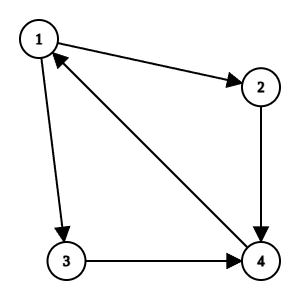
\includegraphics[width=0.28\linewidth]{figures/graph.png}
    \legend{Fonte: Elaborada pelo autor}
    \label{fig:grafo_direcionado}
\end{figure}

\begin{figure}[htbp]
    \centering
    \caption{Exemplo de representação de grafo não direcionado conexo.}
    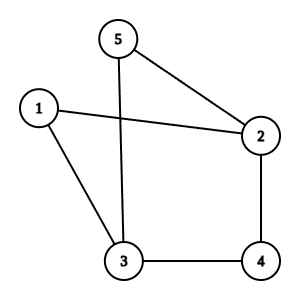
\includegraphics[width=0.28\linewidth]{figures/graph_2.png}
    \legend{Fonte: Elaborada pelo autor}
    \label{fig:grafo_nao_direcionado}
\end{figure}

Já a Figura~\ref{fig:exemplo_figura_externa} ilustra um exemplo de ilustração extraída ou adaptada de \textbf{outro autor}, na qual a fonte explicita a citação e a página de referência:

\begin{figure}[htbp]
    \centering
    \caption{Visão conceitual da estrutura e taxonomia de bancos de dados em grafos.}
    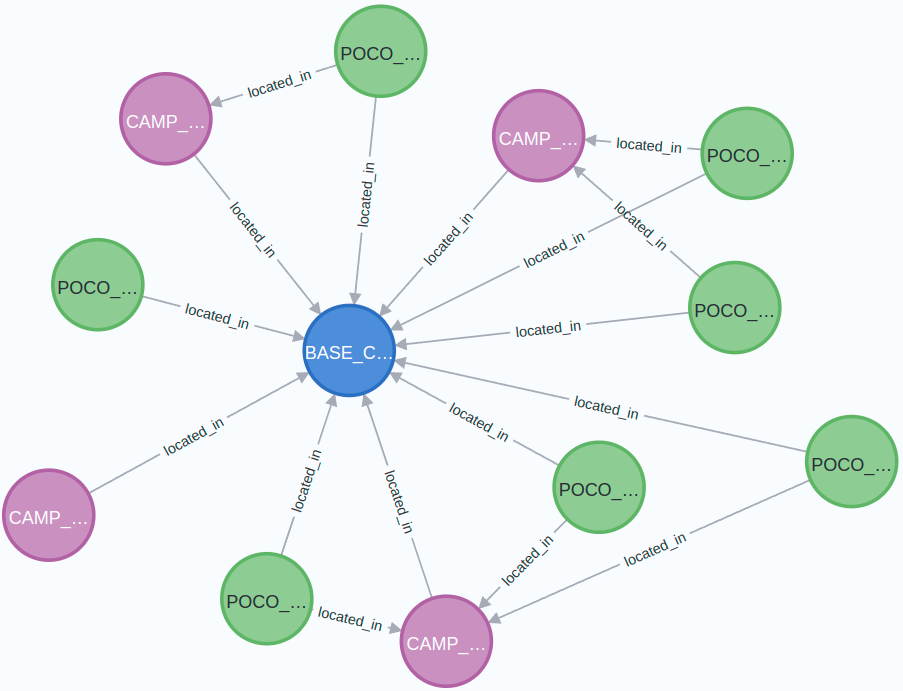
\includegraphics[width=0.72\linewidth]{figures/nodes.png}
    \legend{Fonte: Adaptada de \textcite[p.~10]{besta2023demystifying}}
    \label{fig:exemplo_figura_externa}
\end{figure}

\section{Boas Práticas para Construção de Tabelas}
\label{sec:tabelas_regras}

Analogamente às ilustrações, as tabelas também devem seguir as padronizações das normas de apresentação tabular do IBGE e da ABNT:
\begin{itemize}
    \item \textbf{Título no topo}: A identificação e título (\texttt{\string\caption}) ficam na parte \textbf{superior};
    \item \textbf{Laterais abertas}: As tabelas não devem possuir traços verticais delimitadores nas extremidades laterais externas;
    \item \textbf{Autoria e fonte obrigatórias}: Toda tabela deve explicitar a respectiva fonte na parte inferior (\texttt{\string\legend} ou \texttt{\string\fonte}), mesmo quando construída pelo próprio autor a partir de dados colhidos em sua pesquisa;
    \item \textbf{Tabela de outro autor}: Caso os dados ou a tabela tenham sido extraídos de fonte secundária ou bibliográfica, a indicação de autoria deve citar o autor, o ano e a página exata da publicação.
\end{itemize}

A Tabela~\ref{tab:exemplo_tabela_autor} apresenta um exemplo de tabela de autoria própria sintetizada a partir da literatura:

\begin{table}[htbp]
    \centering
    \caption{Comparativo conceitual de modelos de armazenamento em grafos.}
    \label{tab:exemplo_tabela_autor}
    \begin{tabular}{p{3.5cm}p{5.0cm}p{4.5cm}}
        \toprule
        \textbf{Modelo} & \textbf{Estrutura Principal} & \textbf{Vantagem Central} \\
        \midrule
        LPG (\textit{Labeled Property Graph}) & Nós e arestas com atributos & Flexibilidade e indexação rica \\
        RDF (\textit{Resource Description Framework}) & Triplas sujeito-predicado-objeto & Interoperabilidade semântica \\
        Hipergrafo & Arestas conectando múltiplos nós & Relações de ordem superior ($N$-árias) \\
        \bottomrule
    \end{tabular}
    \legend{Fonte: Elaborada pelo autor}
\end{table}

Por sua vez, a Tabela~\ref{tab:exemplo_tabela_externa} exemplifica uma tabela com dados extraídos diretamente de \textbf{outro autor}, indicando a referência bibliográfica e a página de origem:

\begin{table}[htbp]
    \centering
    \caption{Comparação de características entre bancos relacionais e bancos em grafos.}
    \label{tab:exemplo_tabela_externa}
    \begin{tabular}{p{3.8cm}p{4.5cm}p{4.8cm}}
        \toprule
        \textbf{Critério de Análise} & \textbf{Bancos Relacionais (RDBMS)} & \textbf{Bancos em Grafos} \\
        \midrule
        Modelo de Dados & Tabelas normalizadas (linhas e colunas) & Nós, relacionamentos e propriedades \\
        Navegação entre Relações & Junções de tabelas (\textit{JOINs}) custosas & Travessia direta de ponteiros (\textit{index-free}) \\
        Desempenho em Profundidade & Decai exponencialmente com saltos & Tempo proporcional ao subgrafo explorado \\
        \bottomrule
    \end{tabular}
    \legend{Fonte: Adaptada de \textcite[p.~18]{vukotic2014neo4j}}
\end{table}

% ------------------------------------------------------------------------------
\chapter{Metodologia e Desenvolvimento}
\label{cap:metodologia}

Este capítulo descreve a solução proposta, os métodos de pesquisa, a arquitetura concebida e os detalhes de implementação.

\section{Arquitetura da Solução}
Apresente a visão em alto nível da arquitetura do sistema, diagramas de blocos ou fluxo de dados. Detalhe como as diferentes camadas (ex.: interface, módulo de processamento, banco de dados) se comunicam.

\section{Tecnologias Utilizadas}
Descreva as justificativas técnicas para a escolha das tecnologias e bancos de dados (ex.: Neo4j~\cite{vukotic2014neo4j, Hunger2021}).

\subsection{Consultas Declarativas em Grafos (Cypher)}
Apresente listagens de código quando necessário para ilustrar consultas ou algoritmos fundamentais. Trechos de código devem ser breves e ilustrativos, conforme o Exemplo~\ref{lst:cypher}.

\begin{lstlisting}[language=SQL, caption={Exemplo de consulta em linguagem Cypher para busca de nós vizinhos.}, label={lst:cypher}]
// Busca nos conectados a entidade 'UFRGS' por relacao de cooperacao
MATCH (u:Instituicao {nome: 'UFRGS'})-[r:COOPERA_COM]->(parceiro:Instituicao)
RETURN parceiro.nome AS Nome, r.ano_inicio AS Inicio
ORDER BY Inicio DESC
LIMIT 5;
\end{lstlisting}

% ------------------------------------------------------------------------------
\chapter{Avaliação Experimental e Resultados}
\label{cap:experimentos}

Nenhum trabalho em computação está completo sem avaliação metódica. Este capítulo deve demonstrar cientificamente se os objetivos propostos no Capítulo~\ref{cap:introducao} foram plenamente atingidos.

\section{Planejamento Experimental}
Especifique:
\begin{itemize}
    \item O conjunto de dados (\emph{dataset}) utilizado, sua proveniência e volumetria;
    \item As métricas quantitativas de desempenho (ex.: tempo de resposta, acurácia, revocação, F1-Score);
    \item As configurações de \emph{hardware} e \emph{software} para garantir a reprodutibilidade.
\end{itemize}

\section{Apresentação dos Resultados em Tabelas}
\label{sec:tabelas_experimentos}

A Tabela~\ref{tab:desempenho_consultas} exemplifica a comparação quantitativa de tempo de resposta entre diferentes abordagens avaliadas no experimento. Note a formatação limpa das colunas e o alinhamento numérico.

\begin{table}[htbp]
    \centering
    \caption{Comparação de tempo médio de execução e desvio-padrão entre métodos.}
    \label{tab:desempenho_consultas}
    \begin{tabular}{lccc}
        \toprule
        \textbf{Abordagem} & \textbf{Tempo (ms)} & \textbf{Desvio-Padrão} & \textbf{Acurácia (\%)} \\
        \midrule
        Consulta Relacional Direta     & 342,5 & $\pm 18,2$ & 81,4 \\
        Busca Semântica Simples        & 198,3 & $\pm 12,0$ & 87,9 \\
        Abordagem Proposta (Grafo + IA) & \textbf{76,8} & $\pm \phantom{0}4,5$  & \textbf{95,2} \\
        \bottomrule
    \end{tabular}
    \legend{Fonte: Elaborada pelo autor com base nos experimentos}
\end{table}

A Tabela~\ref{tab:perguntas_amostra} apresenta outro exemplo, com coluna formatada como parágrafo de largura fixa (\texttt{p\{...\}}) para textos descritivos longos.

\begin{table}[htbp]
    \centering
    \caption{Amostra de perguntas do domínio avaliadas pelo sistema.}
    \label{tab:perguntas_amostra}
    \begin{tabular}{cp{10.5cm}}
        \toprule
        \textbf{Categoria} & \textbf{Enunciado da Pergunta de Teste} \\
        \midrule
        Factual & Quais são os departamentos vinculados ao Instituto de Informática da UFRGS? \\
        Factual & Qual docente ministra a disciplina de Redes de Computadores? \\
        Descritiva & Como o sistema integra bancos relacionais legados a grafos de conhecimento? \\
        \bottomrule
    \end{tabular}
    \legend{Fonte: Elaborada pelo autor}
\end{table}

\section{Discussão dos Resultados}
Analise criticamente os dados: explique os motivos pelos quais determinado método superou outro, aponte casos de falha (análise de erros) e esclareça eventuais limitações dos experimentos.

% ------------------------------------------------------------------------------
\chapter{Conclusão e Trabalhos Futuros}
\label{cap:conclusao}

A conclusão retoma o problema formulado, faz um balanço das contribuições alcançadas e discute desdobramentos futuros.

Recapitule sucintamente os pontos-chave:
\begin{itemize}
    \item O trabalho cumpriu os objetivos delineados no Capítulo~\ref{cap:introducao}?
    \item Quais foram as principais contribuições técnicas ou teóricas entregues?
    \item Quais foram os aprendizados e dificuldades encontradas durante a execução?
    \item Quais são as limitações do trabalho?
\end{itemize}

Indique oportunidades reais de continuidade para futuros alunos ou pesquisadores da área:
\begin{enumerate}
    \item Investigar a aplicação de modelos compactos para execução em dispositivos móveis ou \emph{edge computing};
    \item Expandir a base de conhecimento com dados multilíngues;
    \item Conduzir testes com usuários finais para validar a usabilidade do sistema em ambiente de produção.
\end{enumerate}

% ==============================================================================
% 3. ELEMENTOS PÓS-TEXTUAIS
% ==============================================================================
% Incluem:
%   - Referências (obrigatório)
%   - Apêndices (opcional): textos ou documentos elaborados pelo próprio autor
%   - Anexos (opcional): textos ou documentos não elaborados pelo autor
% ==============================================================================

% Imprime as referências bibliográficas com cabeçalho formatado pelo iiufrgs
\printbibliography

% ------------------------------------------------------------------------------
% Apêndices (opcional)
% ------------------------------------------------------------------------------
\appendix

\chapter{Instrumento de Coleta de Dados}
\label{apendice:questionario}

Os apêndices contêm materiais complementares elaborados pelo próprio autor do trabalho (ex.: questionários, detalhamentos de provas matemáticas, esquemáticos de circuitos ou listagens extensas de código).

\section{Roteiro de Entrevista com Usuários}
Apresenta-se aqui o roteiro qualitativo utilizado nas sessões de validação com os participantes voluntários da pesquisa.

% ------------------------------------------------------------------------------
% Anexos (opcional)
% ------------------------------------------------------------------------------
\annex

\chapter{Regulamento de TC do Curso de Ciência da Computação}
\label{anexo:regulamento}

Os anexos reúnem documentos, normas ou textos elaborados por terceiros que servem de fundamentação, comprovação ou ilustração do trabalho (ex.: pareceres de comitê de ética, licenças de bibliotecas, leis ou normas técnicas).

\end{document}
